%%=====tables/model_metrics_heulistic_seg==================================
%% Resultaten
%%=============================================================================

\chapter{\IfLanguageName{dutch}{Resultaten en Evaluatie}{Results and Evaluation}}%
\label{ch:resultaten}

Dit hoofdstuk presenteert de bevindingen van de geconstrueerde Proof of Concept. Een evaluatie van de geïmplementeerde predictieve machine learning-modellen voor de verschillende segmentatie methoden. Ook wordt geconcludeerd wat nog moet gebeuren voor een meerwaarde in het werkveld te bieden.

\section{Data Ingestie}
Hoe kunnen we de data, beschikbaar via het NBB portaal, in een geschikte vorm verkrijgen? De nationale bank van België voorziet verschillende webservices om digitaal te interageren met hun data.
Voor het extraheren van grote hoeveelheden data is er een bulk API beschikbaar, die alle neerleggingen, ingediend op één bepaalde dag, terug geeft in een handig JSON formaat.
Helaas ontrbeekt hier een ondernemingsnummer waardoor deze data nagenoeg nutteloos wordt voor verdere analyse.
Dan blijft enkel de single API over, die per ondernemingsnummer alle beschikbare neergelegde documenten terug geeft. Deze blijt wel over alle nodige data te beschikken maar moet één voor één aangeroepen worden.
Een asynchroon script bleek hier een (weinig performante), maar geschikte oplossing voor een beperkt aantal jaren.
Welk platform gebruiken voor verdere tranformaties en analyses? BigQuery bleek heel geschikt voor de opslag en tranformaties van grote hoeveelheden data, terwijl de kosten heel laag bleven.

\section{Heulistische Segmentatie}
Levert een op regels gebaseerd (heuristische) segmentatie betere resultaten op dan een clustering algoritme (k-means)?
Deze segmentatie methodes werden ontwikkeld met het doel een nuttig machine learning algoritme te trainen voor krediet scoring.
De evaluatie van deze methodes is dan ook gelijk gesteld aan de evalutatie van hun resulterende modellen.
Hoeveel segmenten? Heulistische segmentatie op basis van nace code, grootte en model type leverde maar liefst 6314 segmenten op. Dit resulteert in te weinig data per segment, we moeten minder specifiek gaan.
We namen enkele sectoren en modeltypes samen. Zo bekomen we nog 32 groepen waarvan de grootste voldoende data hebben voor een modeltraining.
\linebreak
Als benchmark trainen we een XGBoost model zonder segmentatie. Dit zal uiteindelijk zelf segmenteren. We bekomen volgende resultaten:
\begin{table}[htbp]
    \small
    \caption{XGBoost model metrics zonder voorafgaande segmentatie}
    \label{tab:model_metrics_no_seg}
    \begin{tabular}{llllllllllllll}
    \toprule

    \textbf{trial id} &
    \textbf{precision} &
    \textbf{recall} &
    \textbf{accuracy} &
    \textbf{f1 score} &
    \textbf{log loss} &
    \textbf{roc auc} \\
    \midrule

    \multicolumn{1}{l}{1} &
    \multicolumn{1}{r}{0.6276} &
    \multicolumn{1}{r}{0.8838} &
    \multicolumn{1}{r}{0.8917} &
    \multicolumn{1}{r}{0.7340} &
    \multicolumn{1}{r}{0.2662} &
    \multicolumn{1}{r}{0.9586} \\
    \bottomrule

\end{tabular}

\end{table}

Volgende paramaters blijken het meeste effect op de accuracy score te hebben:

\begin{table}[htbp]
    \small
    \caption{Feature importance XGBoost model zonder voorafgaande segmentatie}
    \label{tab:feature_importance_no_seg}
    \begin{tabular}{lrr} % l=links, r=rechts (cijfers staan best rechts voor leesbaarheid)
    \toprule
    \textbf{feature}      & \textbf{importance weight} & \textbf{importance gain} \\
    \midrule
    solvency\_y2          & 78.00                        & 1,382.15                   \\
    liquidity\_custom\_y2 & 50.00                        & 638.79                     \\
    equity\_y2            & 114.00                       & 294.75                     \\
    debt\_to\_equity\_y2  & 60.00                        & 181.28                     \\
    roa\_y2               & 58.00                        & 169.90                     \\
    raw\_model\_type      & 74.00                        & 116.58                     \\
    roe\_y2               & 94.00                        & 72.23                      \\
    net\_profit\_y2       & 42.00                        & 49.34                      \\
    equity\_y1            & 38.00                        & 49.23                      \\ % <--- De extra \\ hier lost de error op
    \bottomrule
\end{tabular}
\end{table}

Om te zien of voorafgaande sgemtnatie effect heeft en welke methode de beste is, maakten we gebruik van stratified modeling. We namen de 3 grootste segmenten en trainden hier 3 individuele (in tegenstelling to 1 globaal) XGBoost model op.
Dit waren onze top 3 sectoren (heulistisch gesegmenteerd):
\begin{itemize}
    \item \textbf{diensten/micro}: Deze sector omvat consultancy, it-diensten, enz.
    \item \textbf{handel/micro}: Kleinere winkels en retail.
    \item \textbf{bouw/micro}: Kleinere bouwbedrijven: een kleine loodgieter of aannemer.
  \end{itemize}

Onze drie XGBoostmodellen toonden hogere gemiddelde scores:

\begin{table}[htbp]
    \small
    \caption{XGBoost model metrics na sectorale segmentatie (enkel micro ondernemingen)}
    \label{tab:model_metrics_heul_seg}
    \begin{tabular}{lrrrrrr}
    \toprule
    \textbf{sector} & \textbf{precision} & \textbf{recall} & \textbf{accuracy} & \textbf{f1\_score} & \textbf{log\_loss} & \textbf{roc\_auc} \\
    \midrule
    \textbf{diensten} & 0.6826 & 0.8753 & 0.9333 & 0.7670 & 0.1957 & 0.9711 \\
    \textbf{handel}   & 0.7155 & 0.8507 & 0.9388 & 0.7773 & 0.1998 & 0.9688 \\
    \textbf{bouw}     & 0.7136 & 0.8391 & 0.9375 & 0.7713 & 0.1990 & 0.9665 \\
    \bottomrule
\end{tabular}
\end{table}

een beduidende verbetering op de benchmark. Verrassend want wanneer we naar de feature importance kijken van het base model zien we dat model type en sector redelijk laag staan (respectievelijk plaats 7 en 49). Dit betekent dat ze normaal weinig invloed zouden mogen hebben op de resultaten.
Toen je alles op één grote hoop gooide, moest XGBoost constant compromissen sluiten. Een liquiditeitsratio van 0.9 is voor een IT-consultant met enkel debiteuren (Zakelijke Diensten) misschien geen direct probleem, maar voor een aannemer wél. Door het algoritme nu exclusief te trainen op IT'ers en consultants (Micro/Micro), hebben de beslissingsbomen hyper-specifieke regels kunnen ontdekken die puur voor díe sector gelden. De "ruis" van de andere sectoren is weg.

\section{K-means Segmentatie}
De eerste segmentatie op nagenoeg alle data bracht de ondernemingen allemaal samen in 1 bucket; Dit kwam door de grote hoeveelheid ongestandaardizeerde data.
Bij een tweede poding werden enkel belangrijke ratio's weerhouden. Deze werden gewinsorizeerd om extreme uitschieters te normalizeren.
\begin{figure}[htbp]
    \centering
    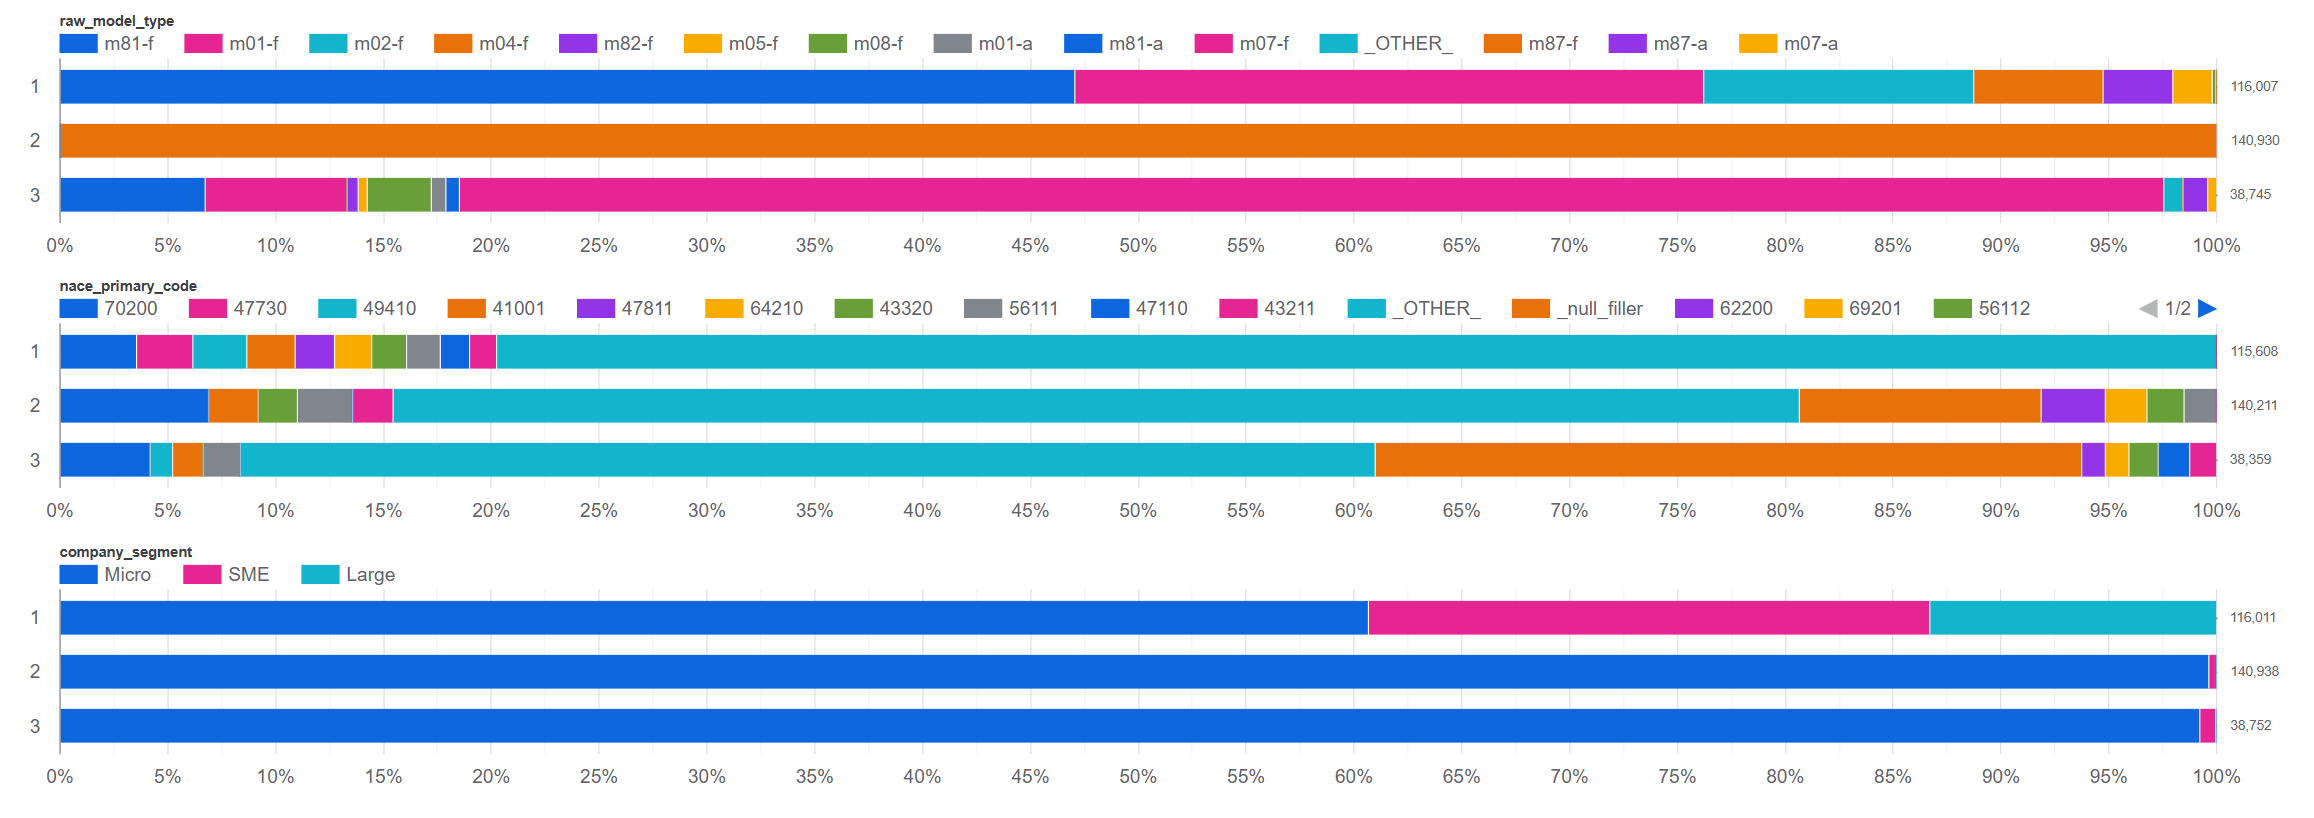
\includegraphics[width=\textwidth]{images/cluster-categories}
    \caption{Verdeling van de verschillende categorische parameters in de clusters}
    \label{fig:cluster-cats}
\end{figure}


\begin{table}[ht]
    \centering
    \caption{K-means Cluster Features}
    \label{tab:features_k_means}
    \resizebox{\textwidth}{!}{ % Dit dwingt de tabel naar de breedte van je tekst
        \begin{table}[ht]
    \centering
    \caption{Overzicht van K-means Centroids en Features (Gefilterd op >5000 ondernemingen)}
    \label{tab:features_k_means}
    \setlength{\tabcolsep}{2pt} % Verkleint de ruimte tussen kolommen om alles te laten passen
    \begin{tabularx}{\textwidth}{@{} r *{10}{X} r @{}}
        \toprule
        \textbf{ID} & \textbf{Rev\_y2} & \textbf{Equity} & \textbf{Profit\_y1} & \textbf{Profit\_y2} & \textbf{$\Delta$Rev} & \textbf{$\Delta$Cust} & \textbf{$\Delta$Inv} & \textbf{$\Delta$Liq\_C} & \textbf{$\Delta$Liq\_S} & \textbf{$\Delta$Supp} & \textbf{Count} \\
        \midrule
        \footnotesize \textbf{9} & 
        \cellcolor[HTML]{F9FCFA}\footnotesize 18.82 & 
        \cellcolor[HTML]{FFFFFF}\footnotesize 106k & 
        \cellcolor[HTML]{FFFFFF}\footnotesize 15k & 
        \cellcolor[HTML]{FFFFFF}\footnotesize 14k & 
        \cellcolor[HTML]{FCFEFD}\footnotesize -6.24 & 
        \cellcolor[HTML]{FDFFFE}\footnotesize -332 & 
        \cellcolor[HTML]{E0F3E9}\footnotesize -1.51 & 
        \footnotesize -0.32 & 
        \cellcolor[HTML]{A8DCC2}\footnotesize 0.38 & 
        \cellcolor[HTML]{F3FBF7}\footnotesize -10.92 & 
        \footnotesize 90163 \\
        
        \footnotesize \textbf{23} & 
        \cellcolor[HTML]{FBFDFC}\footnotesize 18.99 & 
        \cellcolor[HTML]{FAFDFC}\footnotesize 629k & 
        \cellcolor[HTML]{F8FDFA}\footnotesize 82k & 
        \cellcolor[HTML]{F7FCFA}\footnotesize 86k & 
        \cellcolor[HTML]{FEFFFE}\footnotesize -6.30 & 
        \cellcolor[HTML]{FEFFFE}\footnotesize -336 & 
        \cellcolor[HTML]{E0F3E9}\footnotesize -1.52 & 
        \footnotesize -0.24 & 
        \cellcolor[HTML]{FFFFFF}\footnotesize -12.52 & 
        \cellcolor[HTML]{F3FBF7}\footnotesize -10.94 & 
        \footnotesize 44377 \\

        \footnotesize \textbf{10} & 
        \cellcolor[HTML]{E9F6EF}\footnotesize 17.74 & 
        \cellcolor[HTML]{FFFFFF}\footnotesize 156k & 
        \cellcolor[HTML]{FFFFFF}\footnotesize 10k & 
        \cellcolor[HTML]{FFFFFF}\footnotesize 9k & 
        \cellcolor[HTML]{F5FBF8}\footnotesize -5.98 & 
        \cellcolor[HTML]{F9FDFB}\footnotesize -315 & 
        \cellcolor[HTML]{E3F4EB}\footnotesize -2.13 & 
        \footnotesize -0.14 & 
        \cellcolor[HTML]{B8E3CE}\footnotesize -2.07 & 
        \cellcolor[HTML]{F3FBF7}\footnotesize -10.92 & 
        \footnotesize 25842 \\

        \footnotesize 32 & 
        \cellcolor[HTML]{F0F9F5}\footnotesize 18.25 & 
        \cellcolor[HTML]{F3FAF7}\footnotesize 1.4M & 
        \cellcolor[HTML]{F6FCF9}\footnotesize 109k & 
        \cellcolor[HTML]{F6FCF9}\footnotesize 103k & 
        \cellcolor[HTML]{F8FCFA}\footnotesize -6.08 & 
        \cellcolor[HTML]{FFFFFF}\footnotesize -342 & 
        \cellcolor[HTML]{E7F5EE}\footnotesize -2.96 & 
        \footnotesize -0.03 & 
        \cellcolor[HTML]{ACDEC6}\footnotesize -0.32 & 
        \cellcolor[HTML]{F3FBF7}\footnotesize -10.93 & 
        \footnotesize 20178 \\

        \footnotesize 30 & 
        \cellcolor[HTML]{FBFDFC}\footnotesize 18.97 & 
        \cellcolor[HTML]{FFFFFF}\footnotesize 106k & 
        \cellcolor[HTML]{FFFFFF}\footnotesize 13k & 
        \cellcolor[HTML]{FFFFFF}\footnotesize 15k & 
        \cellcolor[HTML]{FDFEFD}\footnotesize -6.25 & 
        \cellcolor[HTML]{F0F9F5}\footnotesize -279 & 
        \cellcolor[HTML]{DAF0E6}\footnotesize -0.36 & 
        \footnotesize -0.28 & 
        \cellcolor[HTML]{9CD7BA}\footnotesize 2.14 & 
        \cellcolor[HTML]{FFFFFF}\footnotesize -11.65 & 
        \footnotesize 15901 \\

        \footnotesize 26 & 
        \cellcolor[HTML]{F6FBF8}\footnotesize 18.62 & 
        \cellcolor[HTML]{DFF2E9}\footnotesize 3.5M & 
        \cellcolor[HTML]{E6F5ED}\footnotesize 276k & 
        \cellcolor[HTML]{E3F4EC}\footnotesize 286k & 
        \cellcolor[HTML]{B6E2CD}\footnotesize -3.75 & 
        \cellcolor[HTML]{57BB8A}\footnotesize 335.15 & 
        \cellcolor[HTML]{D8F0E4}\footnotesize 0.15 & 
        \footnotesize -0.03 & 
        \cellcolor[HTML]{A9DCC3}\footnotesize 0.19 & 
        \cellcolor[HTML]{D2EDE0}\footnotesize -8.95 & 
        \footnotesize 15211 \\

        \footnotesize 18 & 
        \cellcolor[HTML]{57BB8A}\footnotesize 7.80 & 
        \cellcolor[HTML]{57BB8A}\footnotesize 18M & 
        \cellcolor[HTML]{57BB8A}\footnotesize 1.7M & 
        \cellcolor[HTML]{57BB8A}\footnotesize 1.6M & 
        \cellcolor[HTML]{57BB8A}\footnotesize -0.37 & 
        \cellcolor[HTML]{9ED8BC}\footnotesize 50.79 & 
        \cellcolor[HTML]{57BB8A}\footnotesize 27.38 & 
        \footnotesize 0.15 & 
        \cellcolor[HTML]{A9DDC4}\footnotesize 0.14 & 
        \cellcolor[HTML]{57BB8A}\footnotesize -1.76 & 
        \footnotesize 14411 \\

        \footnotesize 27 & 
        \cellcolor[HTML]{FFFFFF}\footnotesize 19.22 & 
        \cellcolor[HTML]{FFFFFF}\footnotesize 162k & 
        \cellcolor[HTML]{FDFFFE}\footnotesize 32k & 
        \cellcolor[HTML]{FDFEFE}\footnotesize 34k & 
        \cellcolor[HTML]{FFFFFF}\footnotesize -6.36 & 
        \cellcolor[HTML]{FFFFFF}\footnotesize -339 & 
        \cellcolor[HTML]{E2F4EB}\footnotesize -1.96 & 
        \footnotesize -0.35 & 
        \cellcolor[HTML]{A0D9BD}\footnotesize 1.55 & 
        \cellcolor[HTML]{F3FBF7}\footnotesize -10.92 & 
        \footnotesize 10584 \\

        \footnotesize 20 & 
        \cellcolor[HTML]{EDF7F2}\footnotesize 18.01 & 
        \cellcolor[HTML]{F5FBF8}\footnotesize 1.2M & 
        \cellcolor[HTML]{EFF9F4}\footnotesize 179k & 
        \cellcolor[HTML]{EDF8F3}\footnotesize 183k & 
        \cellcolor[HTML]{F6FCF9}\footnotesize -6.02 & 
        \cellcolor[HTML]{FAFDFC}\footnotesize -322 & 
        \cellcolor[HTML]{E3F4EC}\footnotesize -2.24 & 
        \footnotesize -0.28 & 
        \cellcolor[HTML]{ACDEC5}\footnotesize -0.20 & 
        \cellcolor[HTML]{F2FAF6}\footnotesize -10.87 & 
        \footnotesize 10051 \\

        \footnotesize 15 & 
        \cellcolor[HTML]{FDFEFE}\footnotesize 19.15 & 
        \cellcolor[HTML]{FFFFFF}\footnotesize 126k & 
        \cellcolor[HTML]{FEFFFE}\footnotesize 25k & 
        \cellcolor[HTML]{FEFFFE}\footnotesize 25k & 
        \cellcolor[HTML]{FFFFFF}\footnotesize -6.33 & 
        \cellcolor[HTML]{FFFFFF}\footnotesize -338 & 
        \cellcolor[HTML]{E2F4EB}\footnotesize -2.02 & 
        \footnotesize -0.29 & 
        \cellcolor[HTML]{AADDC4}\footnotesize 0.12 & 
        \cellcolor[HTML]{F3FBF7}\footnotesize -10.92 & 
        \footnotesize 9633 \\

        \footnotesize 3 & 
        \cellcolor[HTML]{F5FBF8}\footnotesize 18.59 & 
        \cellcolor[HTML]{FFFFFF}\footnotesize 97k & 
        \cellcolor[HTML]{FFFFFF}\footnotesize 7k & 
        \cellcolor[HTML]{FFFFFF}\footnotesize 9k & 
        \cellcolor[HTML]{FFFFFF}\footnotesize -6.34 & 
        \cellcolor[HTML]{F9FDFB}\footnotesize -314 & 
        \cellcolor[HTML]{E2F4EB}\footnotesize -2.00 & 
        \footnotesize -0.19 & 
        \cellcolor[HTML]{57BB8A}\footnotesize 12.17 & 
        \cellcolor[HTML]{F3FBF7}\footnotesize -10.92 & 
        \footnotesize 8788 \\

        \footnotesize 1 & 
        \cellcolor[HTML]{DDF1E7}\footnotesize 16.96 & 
        \cellcolor[HTML]{EEF8F3}\footnotesize 1.9M & 
        \cellcolor[HTML]{FEFFFE}\footnotesize 28k & 
        \cellcolor[HTML]{FFFFFF}\footnotesize 11k & 
        \cellcolor[HTML]{DCF1E7}\footnotesize -5.10 & 
        \cellcolor[HTML]{DBF1E6}\footnotesize -196 & 
        \cellcolor[HTML]{FFFFFF}\footnotesize -8.23 & 
        \footnotesize 1.01 & 
        \cellcolor[HTML]{ACDEC5}\footnotesize -0.24 & 
        \cellcolor[HTML]{F1FAF5}\footnotesize -10.78 & 
        \footnotesize 6734 \\

        \footnotesize 8 & 
        \cellcolor[HTML]{F7FBF9}\footnotesize 18.69 & 
        \cellcolor[HTML]{FFFFFF}\footnotesize 61k & 
        \cellcolor[HTML]{FFFFFF}\footnotesize 13k & 
        \cellcolor[HTML]{FFFFFF}\footnotesize 7k & 
        \cellcolor[HTML]{FBFEFD}\footnotesize -6.20 & 
        \cellcolor[HTML]{FDFEFE}\footnotesize -332 & 
        \cellcolor[HTML]{E2F4EB}\footnotesize -1.95 & 
        \footnotesize -0.28 & 
        \cellcolor[HTML]{ACDEC5}\footnotesize -0.24 & 
        \cellcolor[HTML]{F3FBF7}\footnotesize -10.92 & 
        \footnotesize 5330 \\
        \bottomrule
    \end{tabularx}
\end{table}
    }
\end{table}
We verplichten het model om ook 32 clusters te genereren om een gelijkaardige proefopstelling te garanderen.
Zoals je kan zien in \ref{fig:cluster-cats} wordt er weinig geslecteerd op categorische variabelen. De enigste bepalende factor blijkt het modeltype te zijn.
Een waarneming die we ook tegen kwamen bij het benchmark model, dat de 7e plek innam van paramater importance \ref{tab:feature_importance_no_seg}


\begin{table}[htbp]
    \small
    \caption{XGBoost model metrics na k-means clustering}
    \label{tab:model_merics_k_means}
    \begin{tabular}{rrrrrrr}
    \toprule
    \multicolumn{1}{l}{\textbf{cluster}} &
    \multicolumn{1}{l}{\textbf{precision}} &
    \multicolumn{1}{l}{\textbf{recall}} &
    \multicolumn{1}{l}{\textbf{accuracy}} &
    \multicolumn{1}{l}{\textbf{f1\_score}} &
    \multicolumn{1}{l}{\textbf{log\_loss}} &
    \multicolumn{1}{l}{\textbf{roc\_auc}} \\
    \midrule
    \textbf{1} & 0.5223 & 0.8135 & 0.8553 & 0.6362 & 0.3468 & 0.9257 \\
    \textbf{2} & 0.7141 & 0.9186 & 0.9280 & 0.8035 & 0.1876 & 0.9767 \\
    \textbf{3} & 0.7511 & 0.7957 & 0.8510 & 0.7727 & 0.3704 & 0.9151 \\
    \bottomrule
\end{tabular}

\end{table}

\section{Prestaties van de Machine Learning-modellen}
Om toekomstige kredietrisico's te voorspellen, werden verschillende classificatiemodellen getraind op de geclusterde dataset met behulp van \textit{scikit-learn}. Het doel van de modellen was om op basis van de financiële ratio's uit jaar $X-2$ en $X-1$ een indicatie te geven van financiële distress in jaar $X$.

Er werd een vergelijking gemaakt tussen een traditioneel Logistisch Regressiemodel en een Random Forest-algoritme (een vorm van ensemble learning). Het Random Forest-model presteerde significant beter. Waar de logistieke regressie een nauwkeurigheid (accuracy) behaalde van 73\%, bereikte het Random Forest-model een nauwkeurigheid van 86\%.

Vooral de recall-metriek voor de risicoklasse (het percentage van daadwerkelijk slechte kredieten dat correct werd gedetecteerd door het model) nam sterk toe dankzij de ensemble-methode. Dit ligt in lijn met de bevindingen van \textcite{Moscato2021}, die eveneens aantoonden dat ensemble-modellen superieur zijn bij complexe financiële datasets.